\documentclass[hyperref,]{ctexart}
\usepackage{lmodern}
\usepackage{amssymb,amsmath}
\usepackage{ifxetex,ifluatex}
\usepackage{fixltx2e} % provides \textsubscript
\ifnum 0\ifxetex 1\fi\ifluatex 1\fi=0 % if pdftex
  \usepackage[T1]{fontenc}
  \usepackage[utf8]{inputenc}
\else % if luatex or xelatex
  \ifxetex
    \usepackage{xltxtra,xunicode}
  \else
    \usepackage{fontspec}
  \fi
  \defaultfontfeatures{Mapping=tex-text,Scale=MatchLowercase}
  \newcommand{\euro}{€}
\fi
% use upquote if available, for straight quotes in verbatim environments
\IfFileExists{upquote.sty}{\usepackage{upquote}}{}
% use microtype if available
\IfFileExists{microtype.sty}{%
\usepackage{microtype}
\UseMicrotypeSet[protrusion]{basicmath} % disable protrusion for tt fonts
}{}
\ifxetex
  \usepackage[setpagesize=false, % page size defined by xetex
              unicode=false, % unicode breaks when used with xetex
              xetex]{hyperref}
\else
  \usepackage[unicode=true]{hyperref}
\fi
\usepackage[usenames,dvipsnames]{color}
\hypersetup{breaklinks=true,
            bookmarks=true,
            pdfauthor={Jingwen Yang},
            pdftitle={灵长动物8脑区转录组进化分析},
            colorlinks=true,
            citecolor=blue,
            urlcolor=blue,
            linkcolor=magenta,
            pdfborder={0 0 0}}
\urlstyle{same}  % don't use monospace font for urls
\usepackage{longtable,booktabs}
\usepackage{graphicx,grffile}
\makeatletter
\def\maxwidth{\ifdim\Gin@nat@width>\linewidth\linewidth\else\Gin@nat@width\fi}
\def\maxheight{\ifdim\Gin@nat@height>\textheight\textheight\else\Gin@nat@height\fi}
\makeatother
% Scale images if necessary, so that they will not overflow the page
% margins by default, and it is still possible to overwrite the defaults
% using explicit options in \includegraphics[width, height, ...]{}
\setkeys{Gin}{width=\maxwidth,height=\maxheight,keepaspectratio}
\setlength{\emergencystretch}{3em}  % prevent overfull lines
\providecommand{\tightlist}{%
  \setlength{\itemsep}{0pt}\setlength{\parskip}{0pt}}
\setcounter{secnumdepth}{5}

\title{灵长动物8脑区转录组进化分析}
\author{Jingwen Yang}
\date{2018-10-15}
\usepackage{graphicx}

% Redefines (sub)paragraphs to behave more like sections
\ifx\paragraph\undefined\else
\let\oldparagraph\paragraph
\renewcommand{\paragraph}[1]{\oldparagraph{#1}\mbox{}}
\fi
\ifx\subparagraph\undefined\else
\let\oldsubparagraph\subparagraph
\renewcommand{\subparagraph}[1]{\oldsubparagraph{#1}\mbox{}}
\fi

\begin{document}
\maketitle

{
\setcounter{tocdepth}{2}
\tableofcontents
}
\section{材料与方法}

\subsection{数据介绍}

  在本文中我们选取了四个灵长动物8个脑区的转录组数据。四个灵长动物分别是human(\emph{Homo
sapiens}), chimpanzee(\emph{Pan troglodytes}), gorilla(\emph{Gorilla
gorilla})和gibbon(\emph{Nomascus
leucogenys})。8脑区的分别为DPFC(dorsolateral prefrontal
cortex背外侧前额叶皮层), VPFC( ventrolateral prefrontal cortex
腹外侧前额叶皮层), PMC(premotor cortex 前运动皮层), V1C( primary
visual cortex 初级视觉皮层), ACC(anterior cingulate cortex
前扣带皮层),STR(striatum 纹状体),HIP(hippocampus
海马体),CB(cerebellum小脑)。其中DPFC,VPFC,PMC,
V1C,ACC属于neocortical areas(新皮质区域),STR,HIP属于subcortical
areas(皮质下区域)。CB是小脑。除去gibbon中的8个组织只有1个生物学重复外,其余物种中的8个组织均有2~6个生物学重复。我们使用RPKM值作为基因的表达水平度量。四个灵长动物中共得到27991个one-to-one
orthologous genes。

\hypertarget{house-keeping-gene}{%
\subsection{看家基因(House keeping
gene)数据集}\label{house-keeping-gene}}

  我们选取了文章中所给出的看家基因列表。该数据集给出了一共个3804个human看家基因列表。我们将这3804个基因集与27991个灵长动物one-to-one
orthologous genes取交集,共得到3405个灵长动物看家基因。

\hypertarget{nervous-system-development-gene}{%
\subsection{神经系统发育相关基因(Nervous System development
gene)数据集}\label{nervous-system-development-gene}}

  DAVID数据库中与``Nervous System development''相关的GO Term ID
为GO:0007399,该GO
Term包含个子Term,共包含265个基因。我们将这265个基因集与27991个灵长动物one-to-one
orthologous genes取交集,共得到240个灵长动物神经系统发育相关基因。

\section{结果与讨论}

\subsection{灵长动物不同脑区进化关系}

  我们分析了4个灵长动物8个脑区的转录组数据,共得到了27991个one-to-one
orthologous
genes。我们使用sOU距离计算了表达距离矩阵,并以gibbon的CB组织作为外类群,构建了这些组织的表达特征树,表达特征树的拓扑结构具有较高的Bootstrap值支持,如图一所示。表达特征树的所包含的信息可总结如下:

\begin{enumerate}
\def\labelenumi{\arabic{enumi}.}
\tightlist
\item
  8个脑区中的7个大脑区域在4个灵长动物中分别聚集在一起。而且针对每个物种而言,5个新皮质区域(DPFC,VPFC,PMC,
  V1C,ACC)倾向聚集在一起,2个皮质下区域(STR,HIP)倾向聚集在一起。
\item
  8个脑区中的小脑作为在形态学上与大脑相对独立的组织展现出了其独有的进化特征。就小脑这个组织而言,四个灵长动物的小脑组织在进化树中与大脑各个区域分开,单独聚在一起。
\item
  Gibbon的HIP与其它物种的CB聚集在一起。一方面可能反映出Gibbon的HIP具有独特的进化方式,另一方面可能是由于采样问题而出现的误差。考虑到Gibbon的8个脑区只有一个生物学重复,我们怀疑后一种情况的可能性更大。在后续的工作中我们将尽量避免涉及到Gibbon中HIP的分析。
\end{enumerate}

  灵长动物8个脑区表达特征树的拓扑结构可反映两部分的内容:

\begin{enumerate}
\def\labelenumi{\arabic{enumi}.}
\tightlist
\item
  我们所构建的表达特征树与这些脑区的形态学相似度比较一致。在转录组分析中,我们用于计算表达距离的sOU方法可帮助我们探索比较转录组分析的进化关系。
\item
  不同物种不同组织之间的表达距离由两部分构成,分别是进化距离(evolutionary
  distance)和发育距离(development
  distance)。当不同物种的不同组织之间的进化距离大于发育距离时,同一物种内的不同组织倾向于聚集在一起;而当进化距离小于发育距离时,不同物种的同一组织倾向于聚集在一起。我们构建的灵长动物不同脑区表达特征树反映出(i)针对大脑和小脑这两个组织而言,大脑与小脑之间的进化距离小于发育距离,所以不同物种的同一组织(大脑或小脑)聚集在一起;(ii)就大脑的7个不同区域而言,其发育距离小于其进化距离,所以同一物种内的7个不同大脑区域聚集在一起。值得注意的是,5个新皮质区域的距离和2个皮质下区域的距离要小于两个区域间的距离。
\end{enumerate}

\begin{figure}
\centering
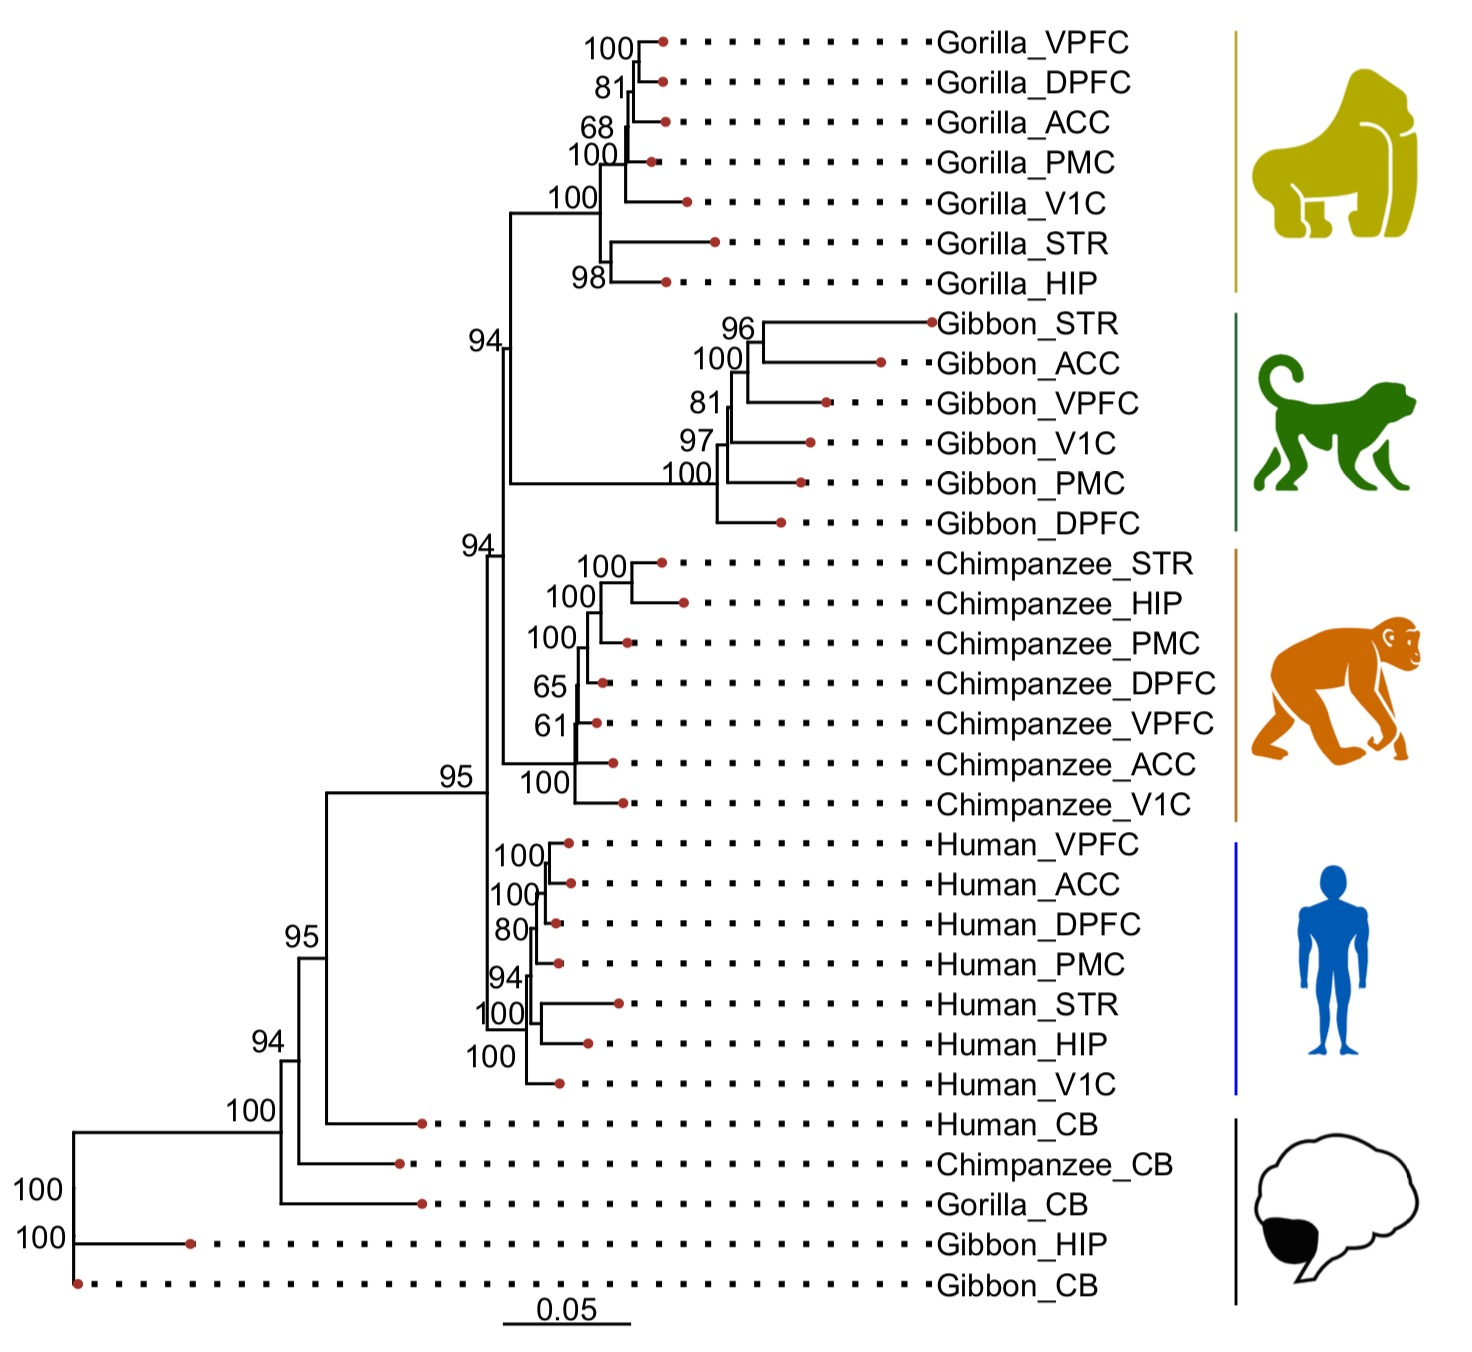
\includegraphics[width=0.8\textwidth,height=0.8\textwidth]{/blog/2018-10-15-transcriptome/fig1.jpg}
\caption{图一 4个灵长动物8个脑区表达进化关系}
\end{figure}

\subsection{8脑区进化速度比较}

  我们同样的计算方法对8个脑区分别计算了其在4个灵长动物中的表达进化距离,并构建了表达特征树。图二表示8个脑区的进化关系图。我们根据四个灵长动物的表达分化时间计算了8个脑区在6个两两物种对中的进化速度。表一列出了8个脑区进化速度的数值,图三表示8个脑区进化速度的散点图。

  就进化关系而言:

\begin{itemize}
\tightlist
\item
  DPFC,VPFC,PMC,V1C这四个组织具有较为一致的进化关系,并与物种的进化关系一致。这种情况也发生在STR和CB这两个组织中。
\item
  值得注意的是,在ACC和HIP这两个组织的表达特征树中,chimpanzee与gorilla聚集在一起,human与这两个物种分开了。而且HIP在不同的物种间具有更大的进化距离。有意思的是,相较于chimpanzee和gorilla,HIP在human中具有更短的进化枝长。
\end{itemize}

  就进化速度而言:

\begin{itemize}
\tightlist
\item
  HIP的进化速度相比于其它脑区的进化速度更快
\item
  HIP在human-lineage中相比chimpanzee-lineage具有更慢的进化速度
\item
  CB的进化速度相比于其它的大脑区域进化速度更慢。
\item
  其它的脑区(如5个新皮质区域)的进化速度处于中间状态,并且相互之间差异不大。
\item
  8个脑区的进化速度的数量级均在\(10^{-9}\)。
\end{itemize}

\begin{longtable}[]{@{}ccccc@{}}
\caption{表一 4个灵长动物物种分化时间(Million Year)}\tabularnewline
\toprule
& Human & Chimpanzee & Gorilla & Gibbon\tabularnewline
\midrule
\endfirsthead
\toprule
& Human & Chimpanzee & Gorilla & Gibbon\tabularnewline
\midrule
\endhead
Human & 0 & & &\tabularnewline
Chimpanzee & 6.4 & 0 & &\tabularnewline
Gorilla & 8.61 & 8.61 & 0 &\tabularnewline
Gibbon & 19.43 & 19.43 & 19.43 & 0\tabularnewline
\bottomrule
\end{longtable}

\begin{figure}
\centering
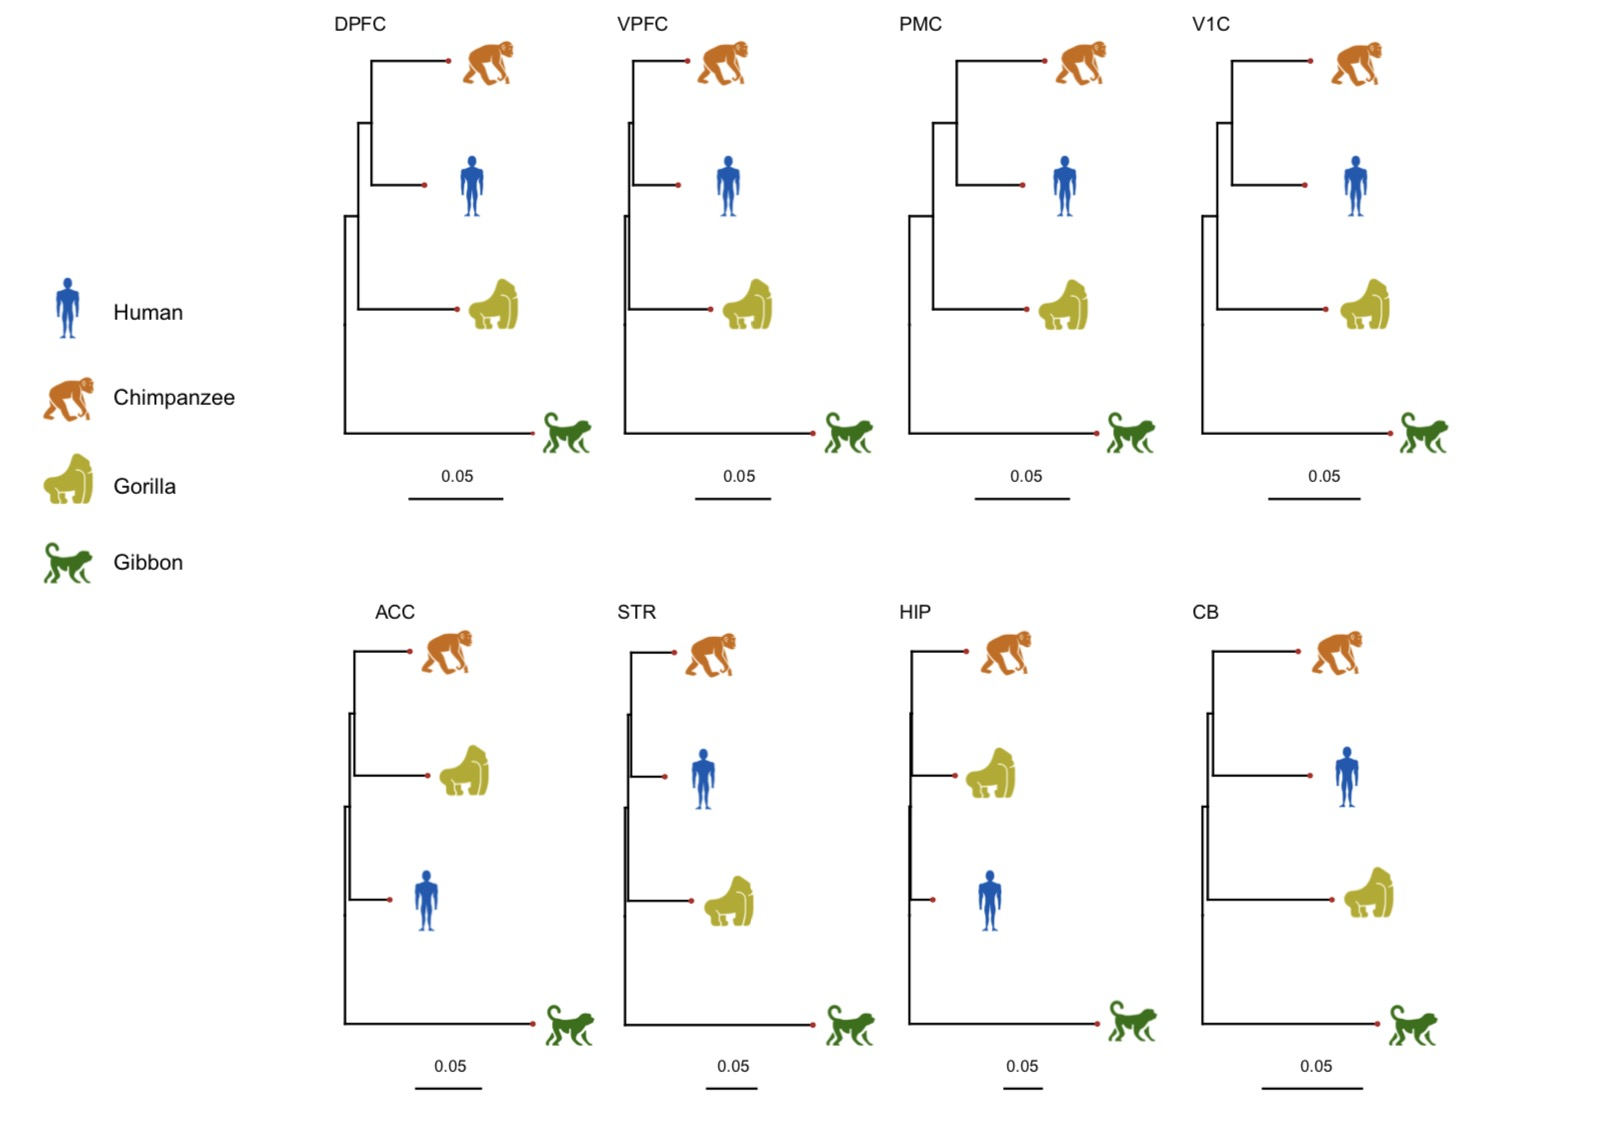
\includegraphics[width=1\textwidth,height=1\textwidth]{/blog/2018-10-15-transcriptom/fig2.jpg}
\caption{图二 8个脑区表达进化关系}
\end{figure}

\begin{figure}
\centering
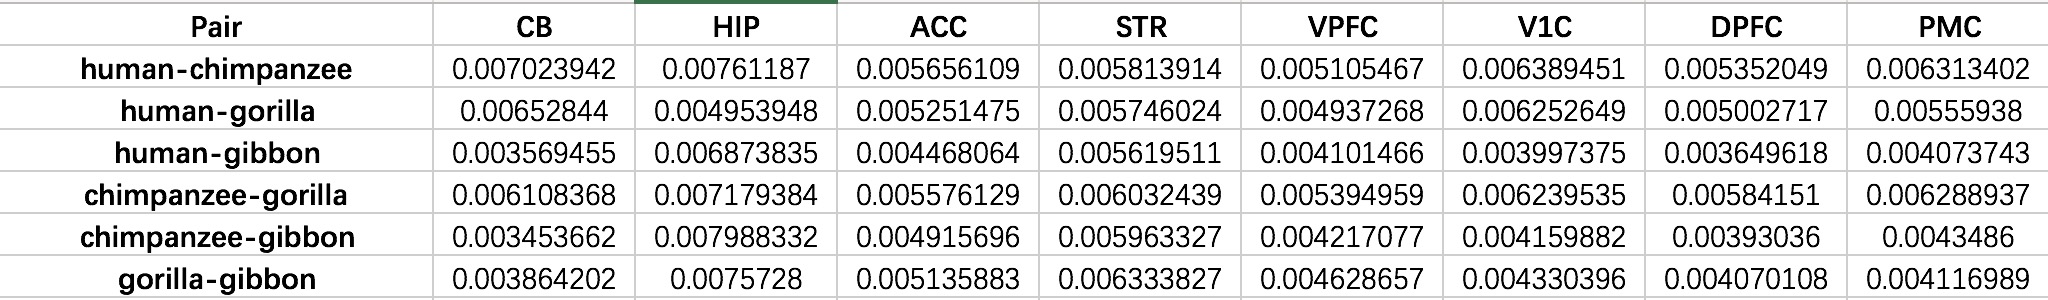
\includegraphics[width=1.2\textwidth,height=1.2\textwidth]{/blog/2018-10-15-transcriptome/table1.jpg}
\caption{表二 8脑区表达进化速度}
\end{figure}

\begin{figure}
\centering
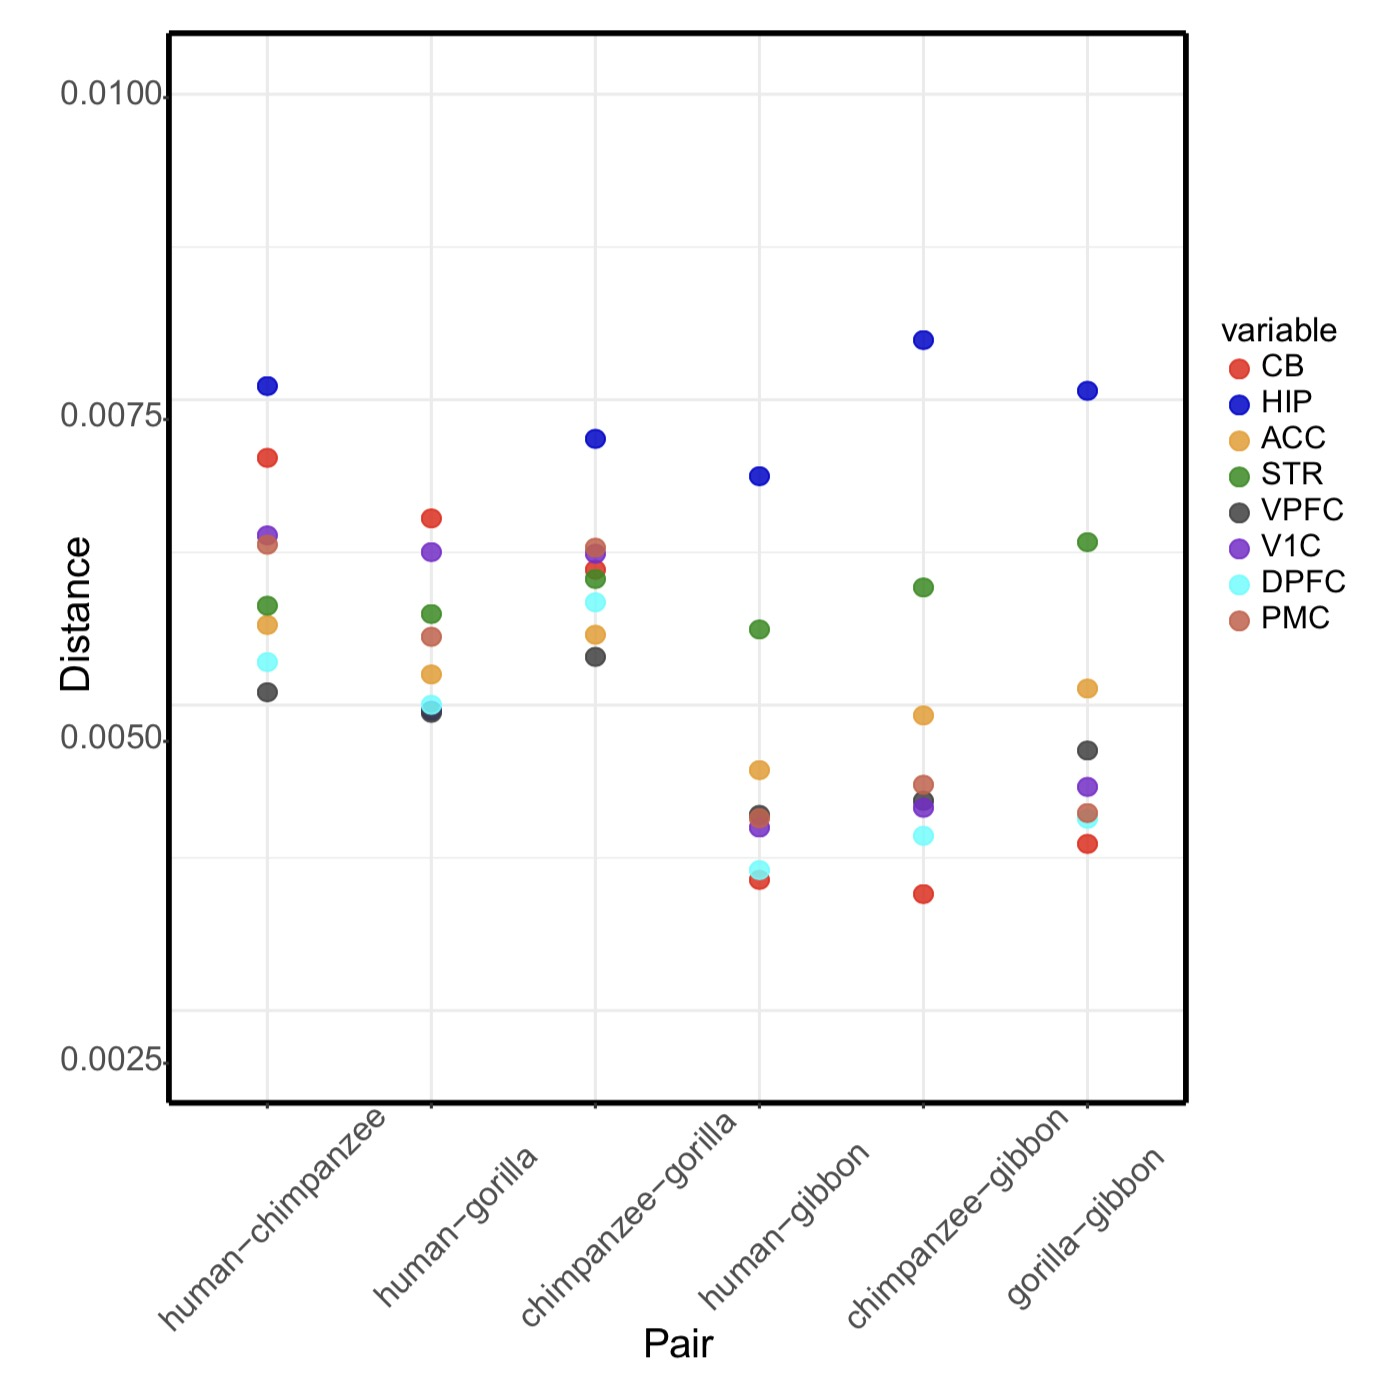
\includegraphics[width=0.7\textwidth,height=0.7\textwidth]{/blog/2018-10-15-transcriptome/fig3.jpg}
\caption{图三 8脑区表达进化速度}
\end{figure}

\hypertarget{kaessmann6}{%
\subsection{Kaessmann数据6个组织在灵长动物中的进化速度}\label{kaessmann6}}

  为了比较本文中灵长动物8个脑区的进化速度与其它组织在灵长动物中的进化速度,我们重新分析了Kaessmann文章中6个组织在6个灵长动物中的进化距离和进化速度。6个灵长动物分别是Human,
Chimanpanzee,Bonobo,Gorilla,Orangutan和Macaque;6个组织分别是brain,cerebellum,heart,liver,kidney以及testis,其中testis在Orangutan物种中缺失。我们共得到13277个one-to-one
orthologous
genes。表三列出了6个灵长动物的物种分化时间;6个组织在两两物种中的进化速度散点图如图四所示。从我们的结果中可以反映出:

\begin{itemize}
\tightlist
\item
  brain和cerebellum两个与神经系统相关的组织在所有的物种对中具有较低的物种进化速度,进化速度的数量级与本文8个脑区的进化速度也基本一致。
\item
  testis的进化速度最快。

  \begin{longtable}[]{@{}ccccccc@{}}
  \caption{表三 6个灵长动物物种分化时间(Million Year)}\tabularnewline
  \toprule
  & Human & Chimpanzee & Bonobo & Gorilla & Orangutan &
  Macaque\tabularnewline
  \midrule
  \endfirsthead
  \toprule
  & Human & Chimpanzee & Bonobo & Gorilla & Orangutan &
  Macaque\tabularnewline
  \midrule
  \endhead
  Human & 0 & &\tabularnewline
  Chimpanzee & 6.4 & 0 &\tabularnewline
  Bonobo & 6.4 & 2.37 & 0 &\tabularnewline
  Gorilla & 8.61 & 8.61 & 8.61 & 0 &\tabularnewline
  Orangutan & 15.2 & 15.2 & 15.2 & 15.2 & 0 &\tabularnewline
  Macaque & 28.1 & 28.1 & 28.1 & 28.1 & 28.1 & 0\tabularnewline
  \bottomrule
  \end{longtable}

  \begin{figure}
  \centering
  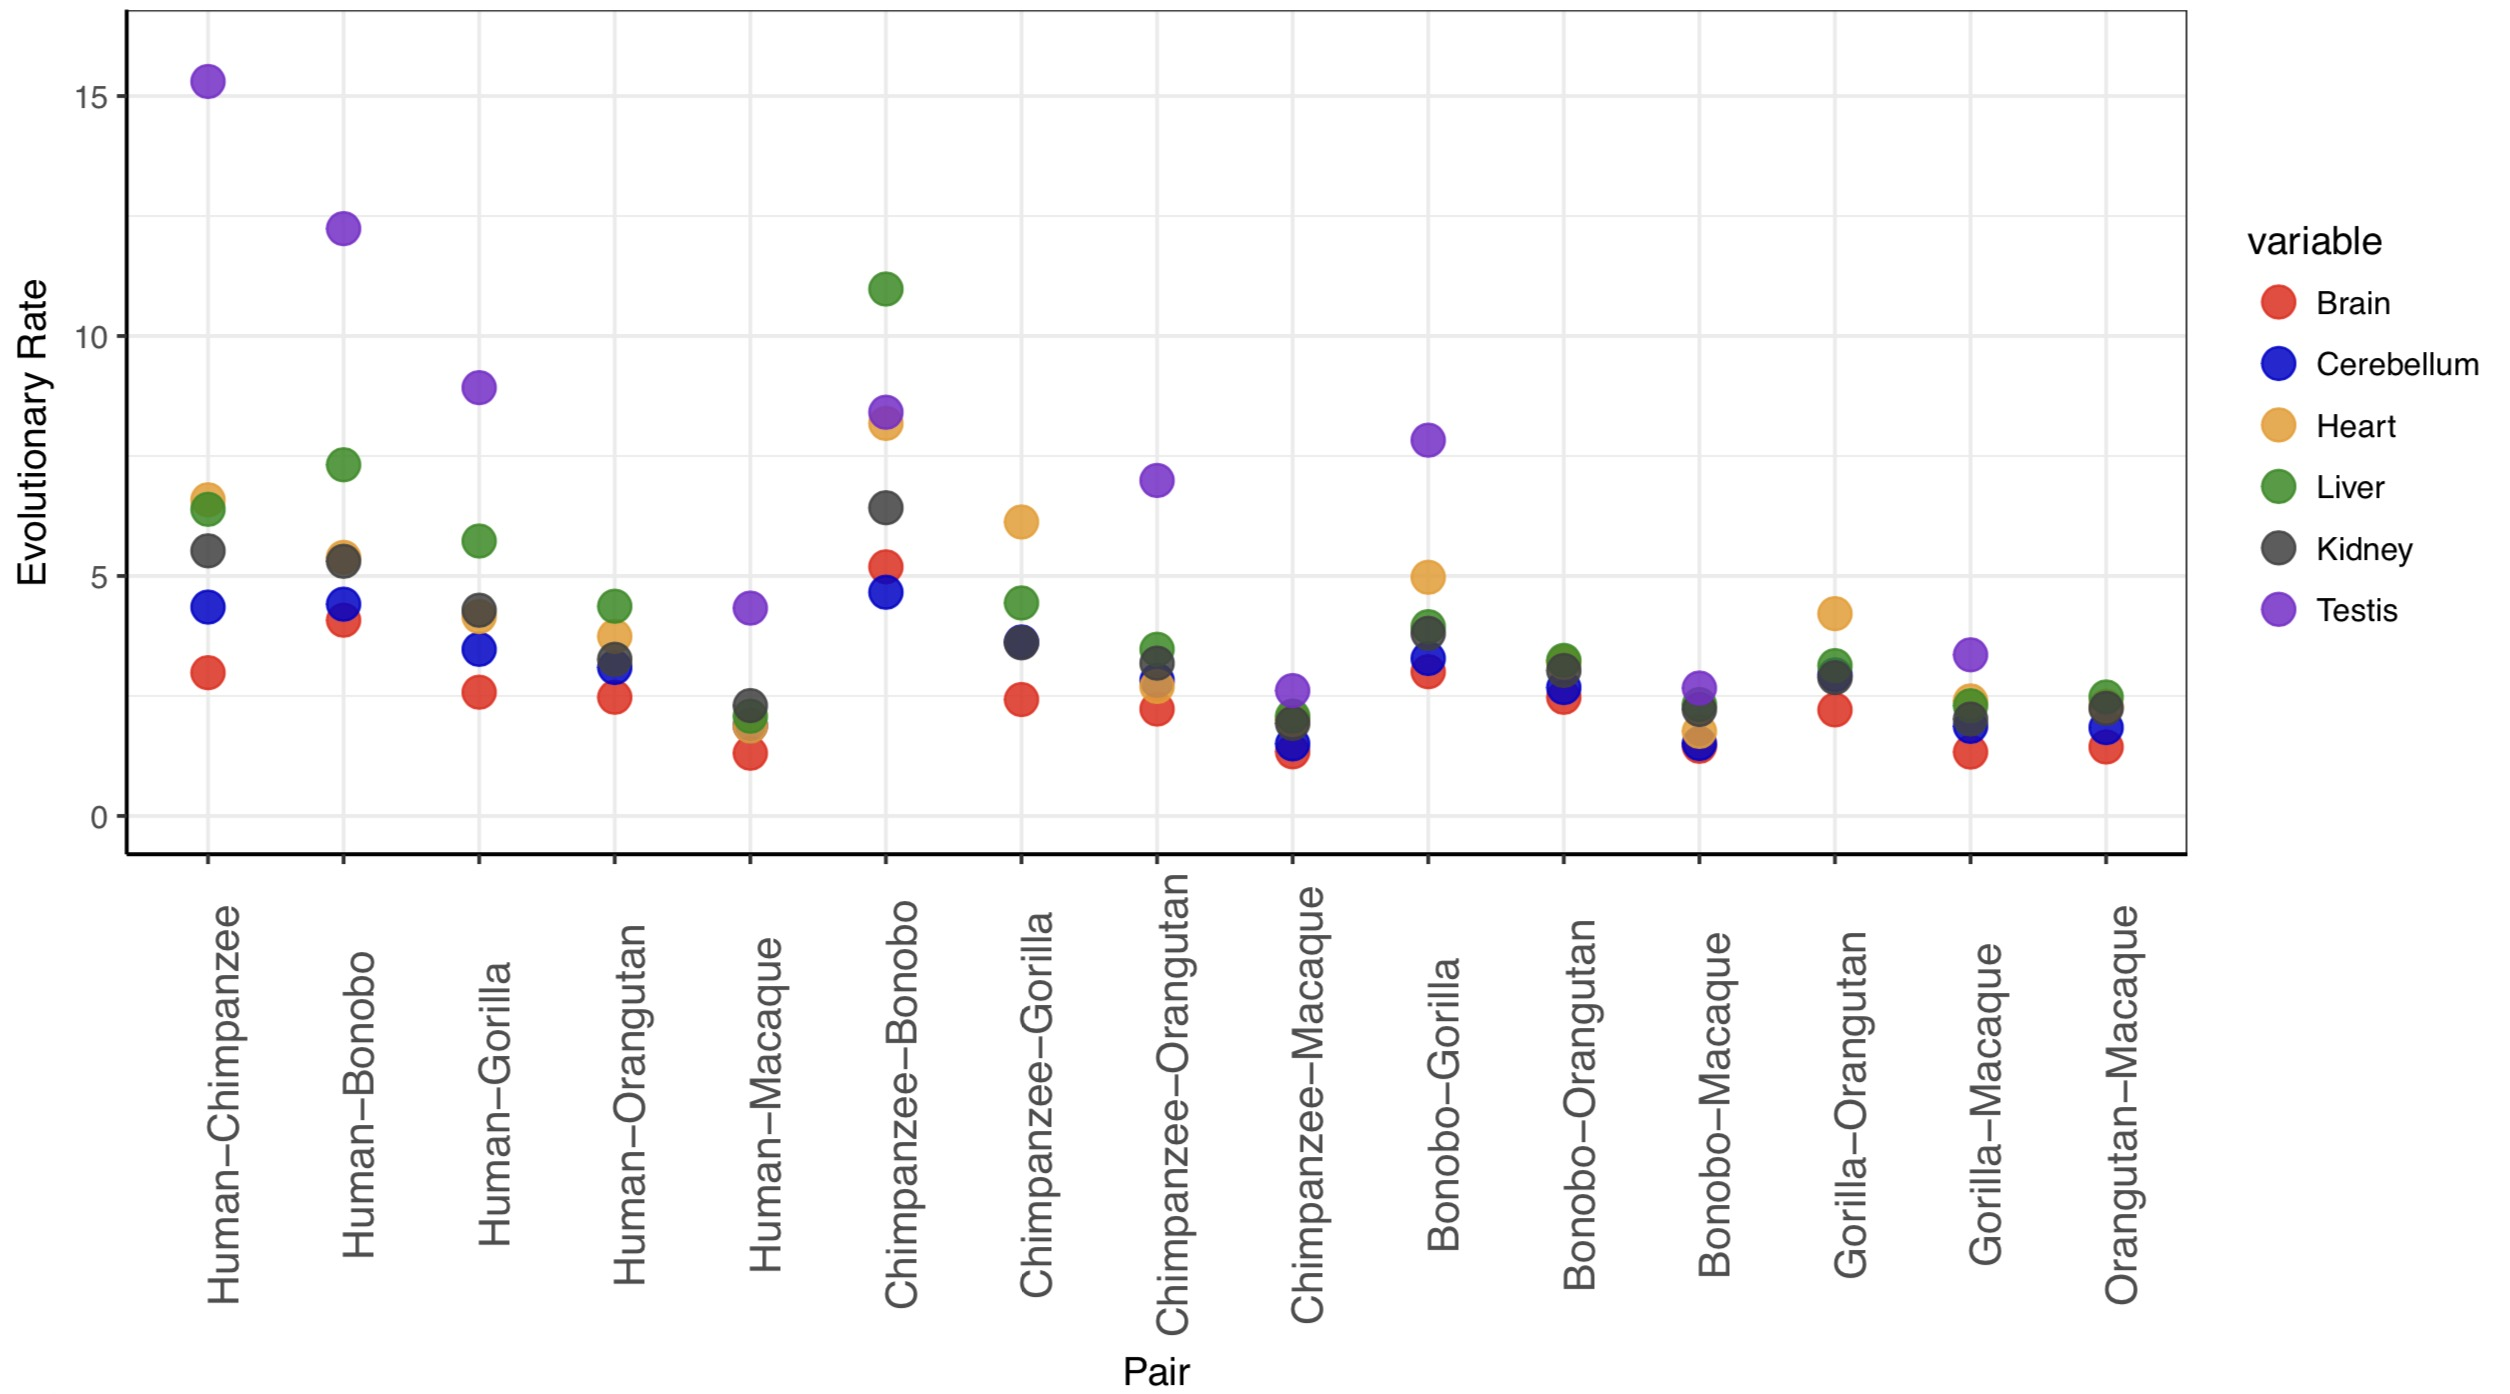
\includegraphics[width=1\textwidth,height=1\textwidth]{/blog/2018-10-15-灵长动物8脑区转录组进化分析_files/Kaessmann进化速度.jpg}
  \caption{图四 Kaessmann数据6个组织在6个灵长动物中的进化速度}
  \end{figure}
\end{itemize}

\subsection{神经系统发育相关基因的进化模式}

  在上文的分析中,我们探究了4个灵长动物8个脑区组织的表达进化模式。我们对27991个one-to-one
orthologous genes
的表达值进行了系统发生分析,我们的结果很好的反映了这些组织整体的进化模式。

  在本小节中,我们希望探究某些具有特殊功能的基因在这8个脑区的进化趋势。为此,我们选取了DAVID数据库中与神经系统发育(Nerve
System Development,简称NSD)相关的GO
term,并得到240个NSD基因进行研究。同时,我们选取了3405个看家基因(HK基因)作为对照。我们分别分析了NSD基因和HK基因中human,chimpanzee,gorilla分别与gibbon在8个脑区中的表达进化距离(图五)。同样做为对照,我们也计算了相同的NDS基因和HK基因在Kaessmann数据中human,chimpanzee,bonobo,gorilla,orangutan分别与macaque在五个组织中的表达进化距离(图六)。

  在图五中,物种间在HIP中相比其它组织具有相当长的进化距离,这可能是由于Gibbon的HIP的样本特异性造成的。对此,我们排除了Gibbon,用同样的数据集重新计算了human,chimpanzee分别与gorilla之间的表达进化距离(图七)。

  在图六中,NSD基因在brain和cerebellum中的的进化距离相比其它非神经系统组织要小,这表明NSD基因主要在神经系统相关组织(brain和cerebellum)中起作用。

  我们的分析结果显示,NSD基因在神经系统相关的组织(Brian,Cerebellum)中相比HK基因具有更短的进化距离,也就是更慢的进化速度。用不同的数据集均得到了一致的结果。这提示,NSD基因作为与神经系统发育密切相关的基因,其功能可能受到了严格的负选择。

  值得注意的是,在HIP中,human与gorilla的距离相比chimpanzee与gorilla之间的距离要短得多。这表明HIP这个组织在human中具有更加缓慢的进化速度。
在物种的进化过程中,某种新功能的获得往往伴随着表达水平的快速进化。而当新功能获得并稳定下来后,在表达上往往会受到严格的负调控。
HIP作为与人类认知和记忆密切相关的组织,在NSD基因中显著的进化速度放缓可能提起其在功能上的重要地位。

\begin{figure}
\centering
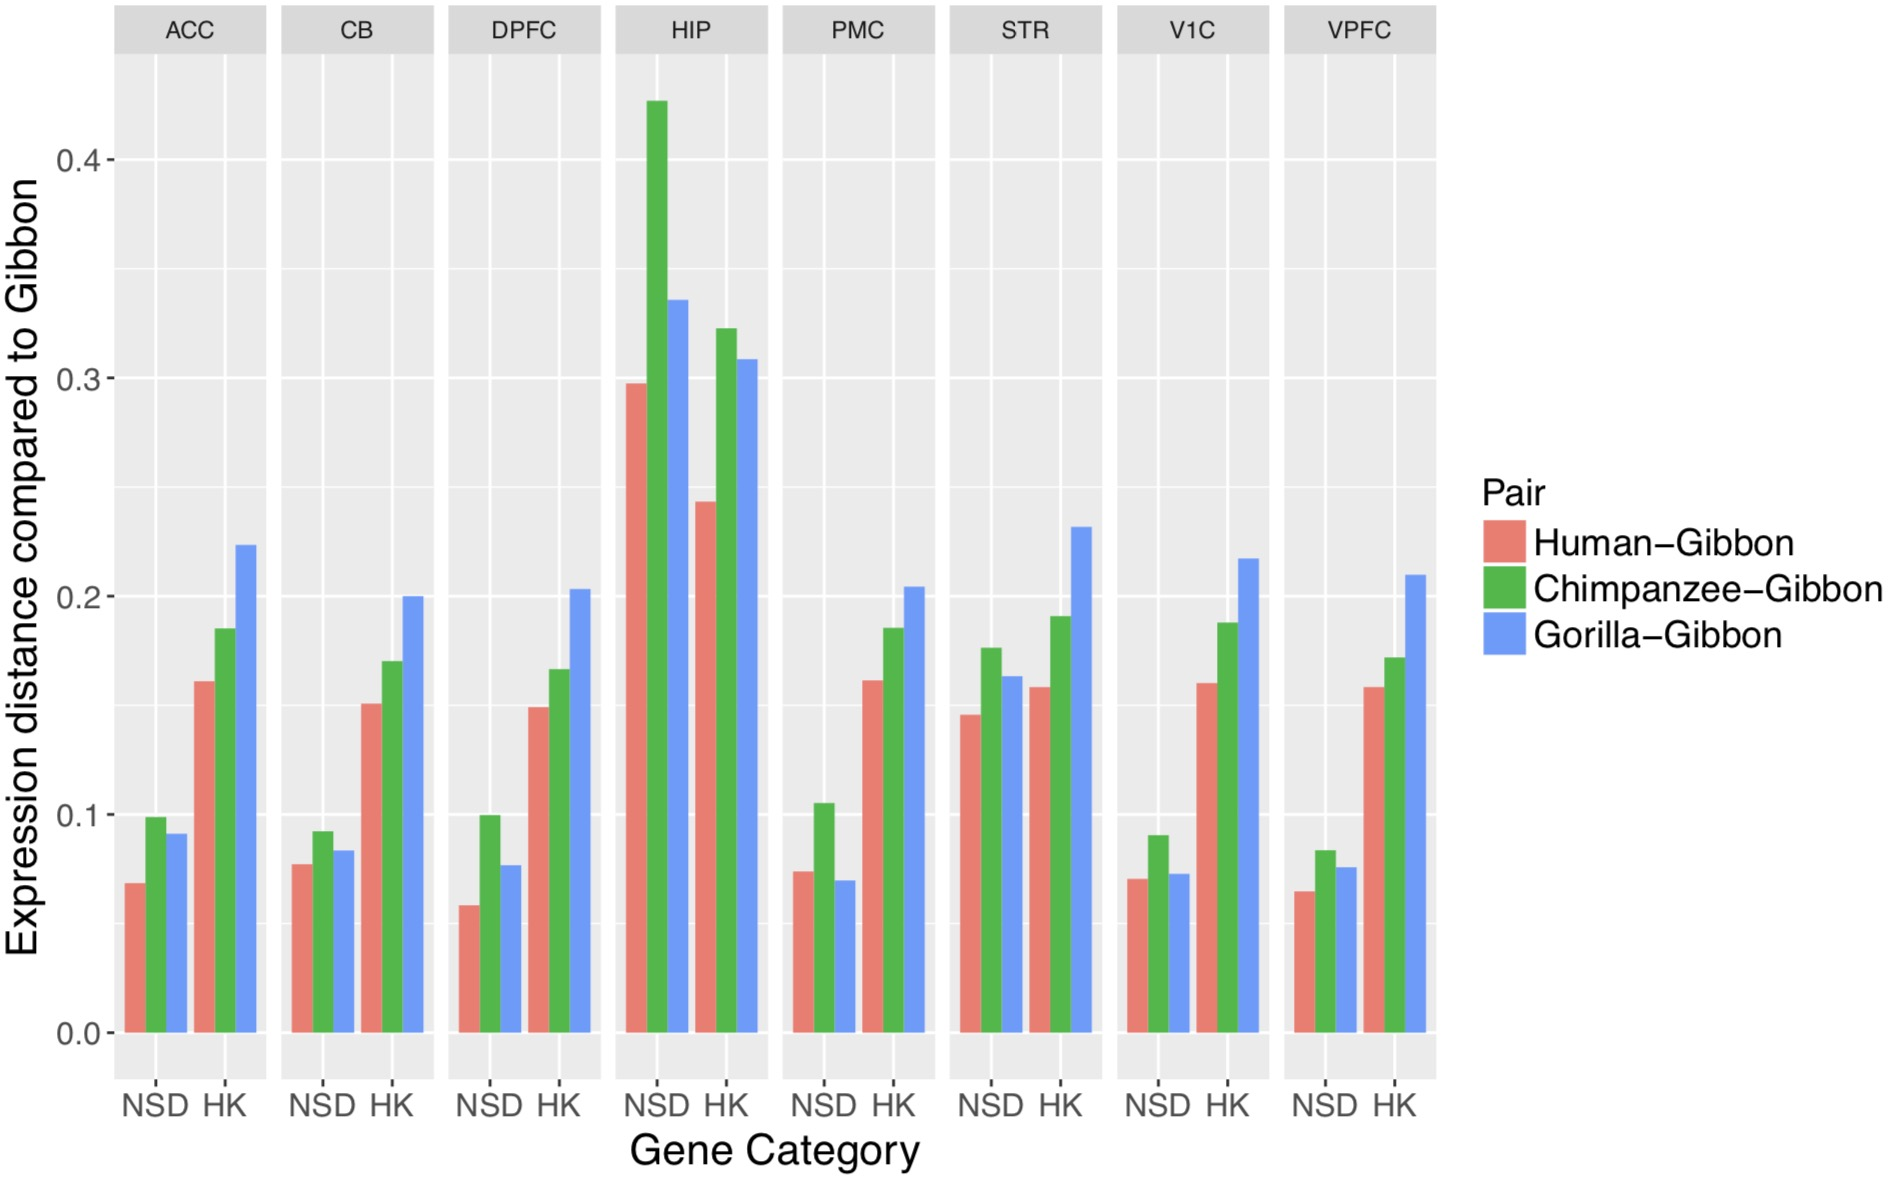
\includegraphics[width=0.8\textwidth,height=0.8\textwidth]{/blog/2018-10-15-灵长动物8脑区转录组进化分析_files/NSD-HK-Gibbon.jpg}
\caption{图五 human, chimpanzee,
gorilla相对gibbon在8个脑区中的表达进化距离}
\end{figure}

\begin{figure}
\centering
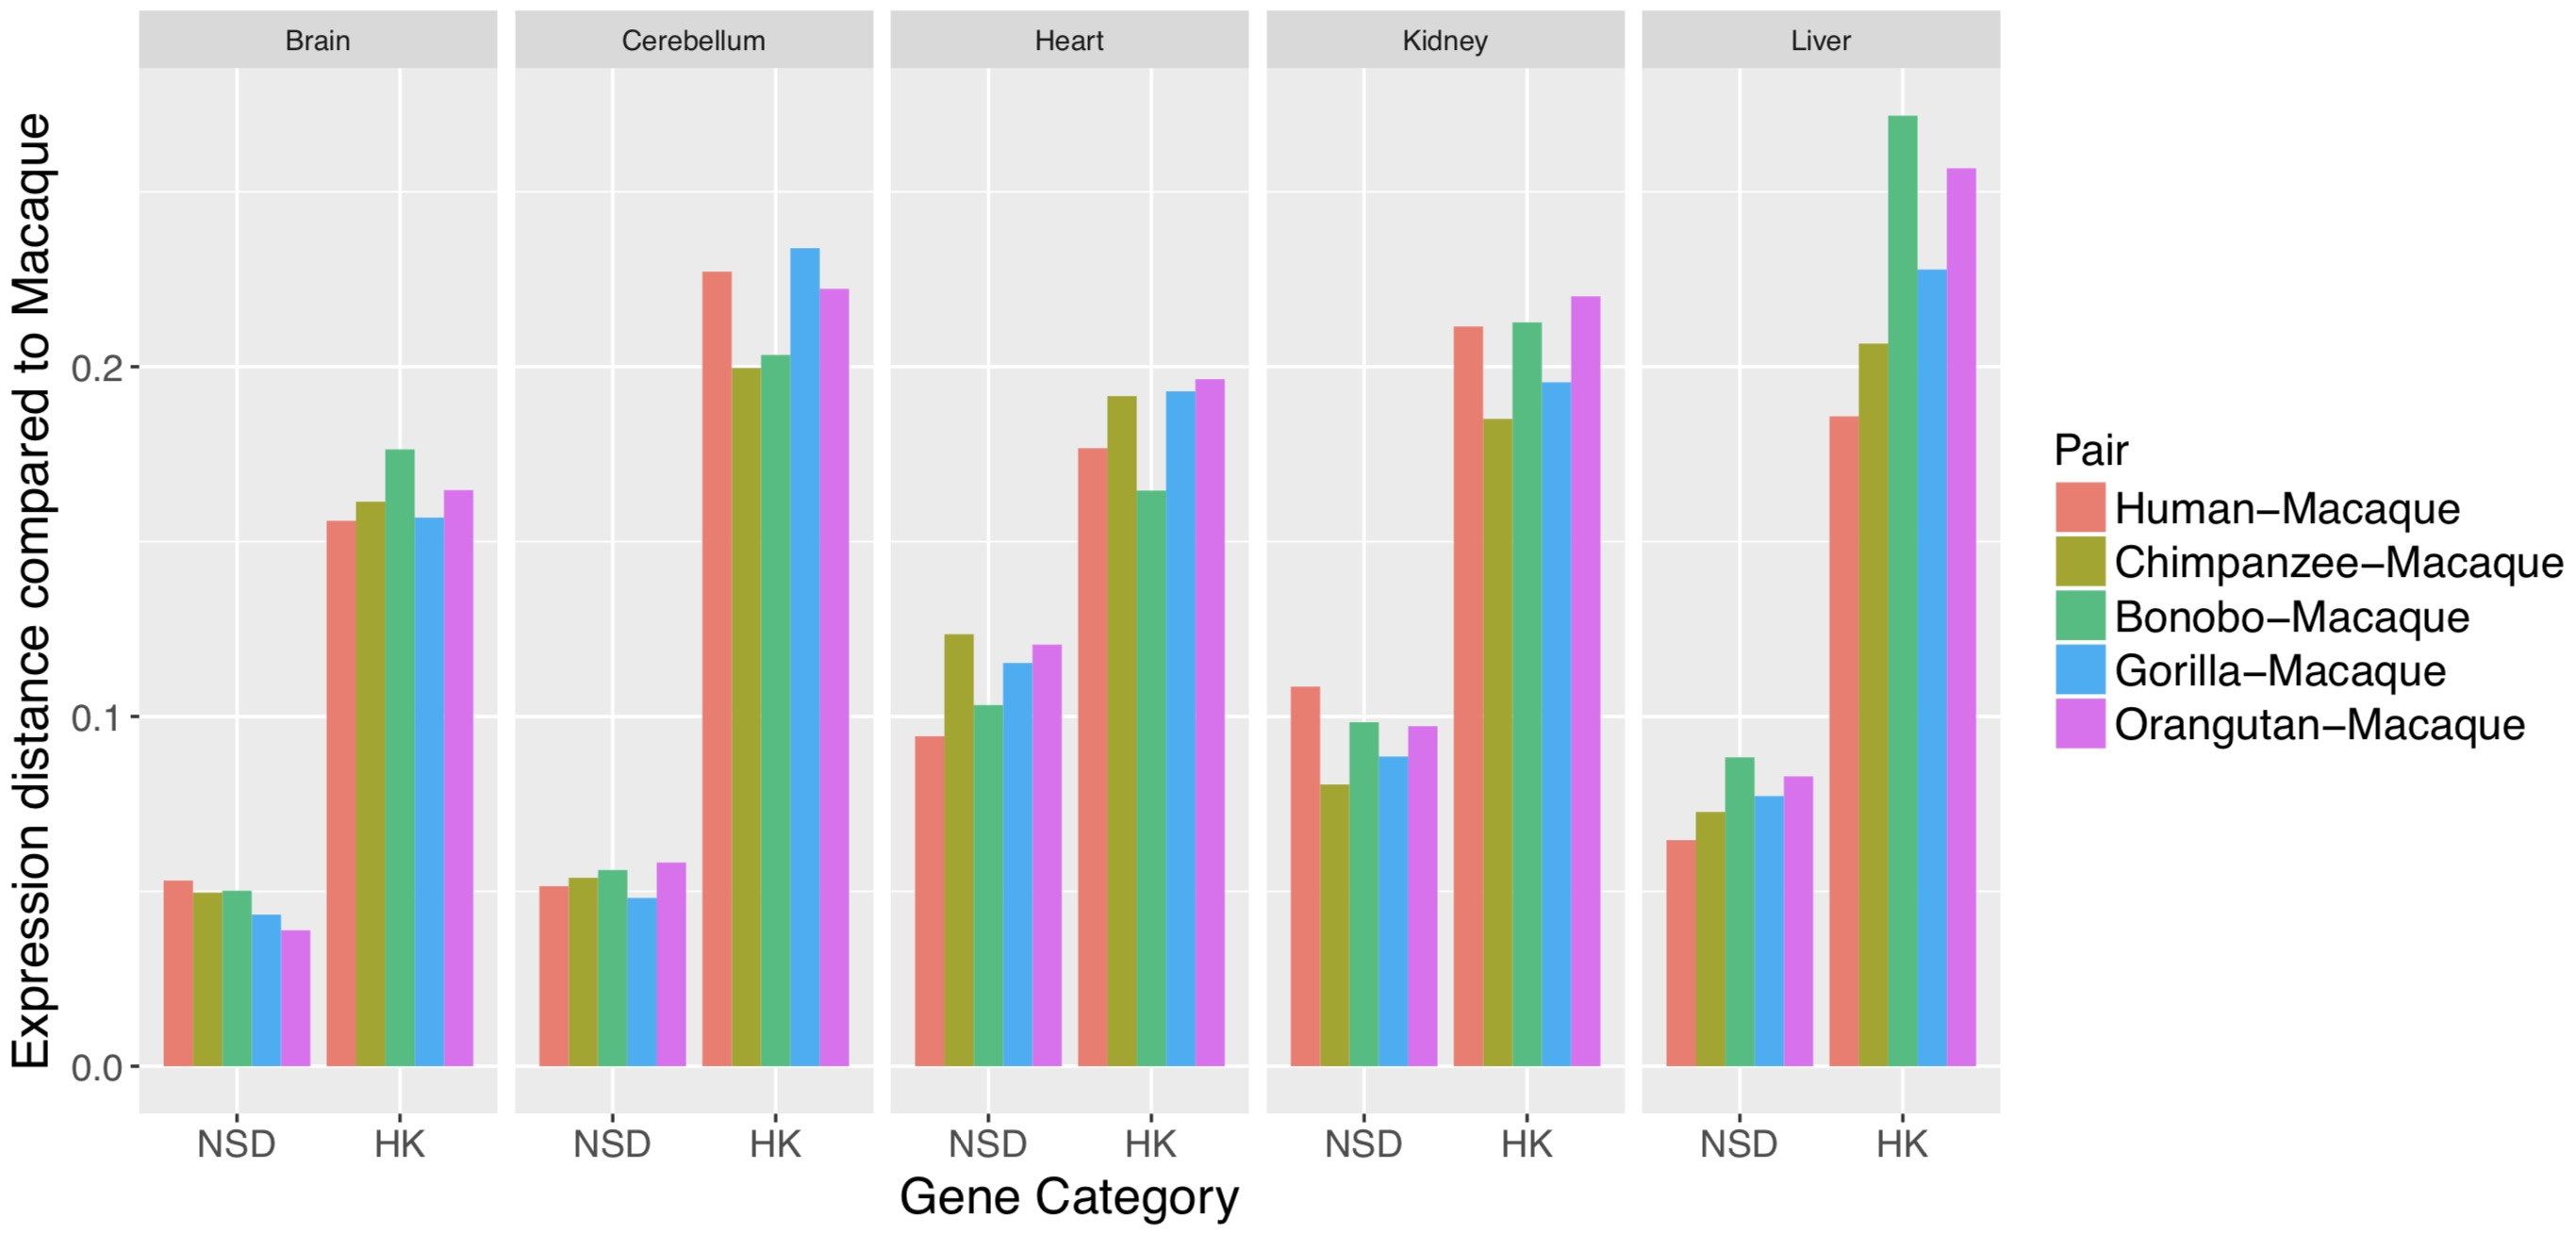
\includegraphics[width=0.8\textwidth,height=0.8\textwidth]{/blog/2018-10-15-灵长动物8脑区转录组进化分析_files/Kaessmann_NSD_HK.jpg}
\caption{图六 human, chimpanzee, bonobo, gorilla,
orangutan相对macaque在brain,cerebellum,liver, heart,
kidney中的表达分化距离}
\end{figure}

\begin{figure}
\centering
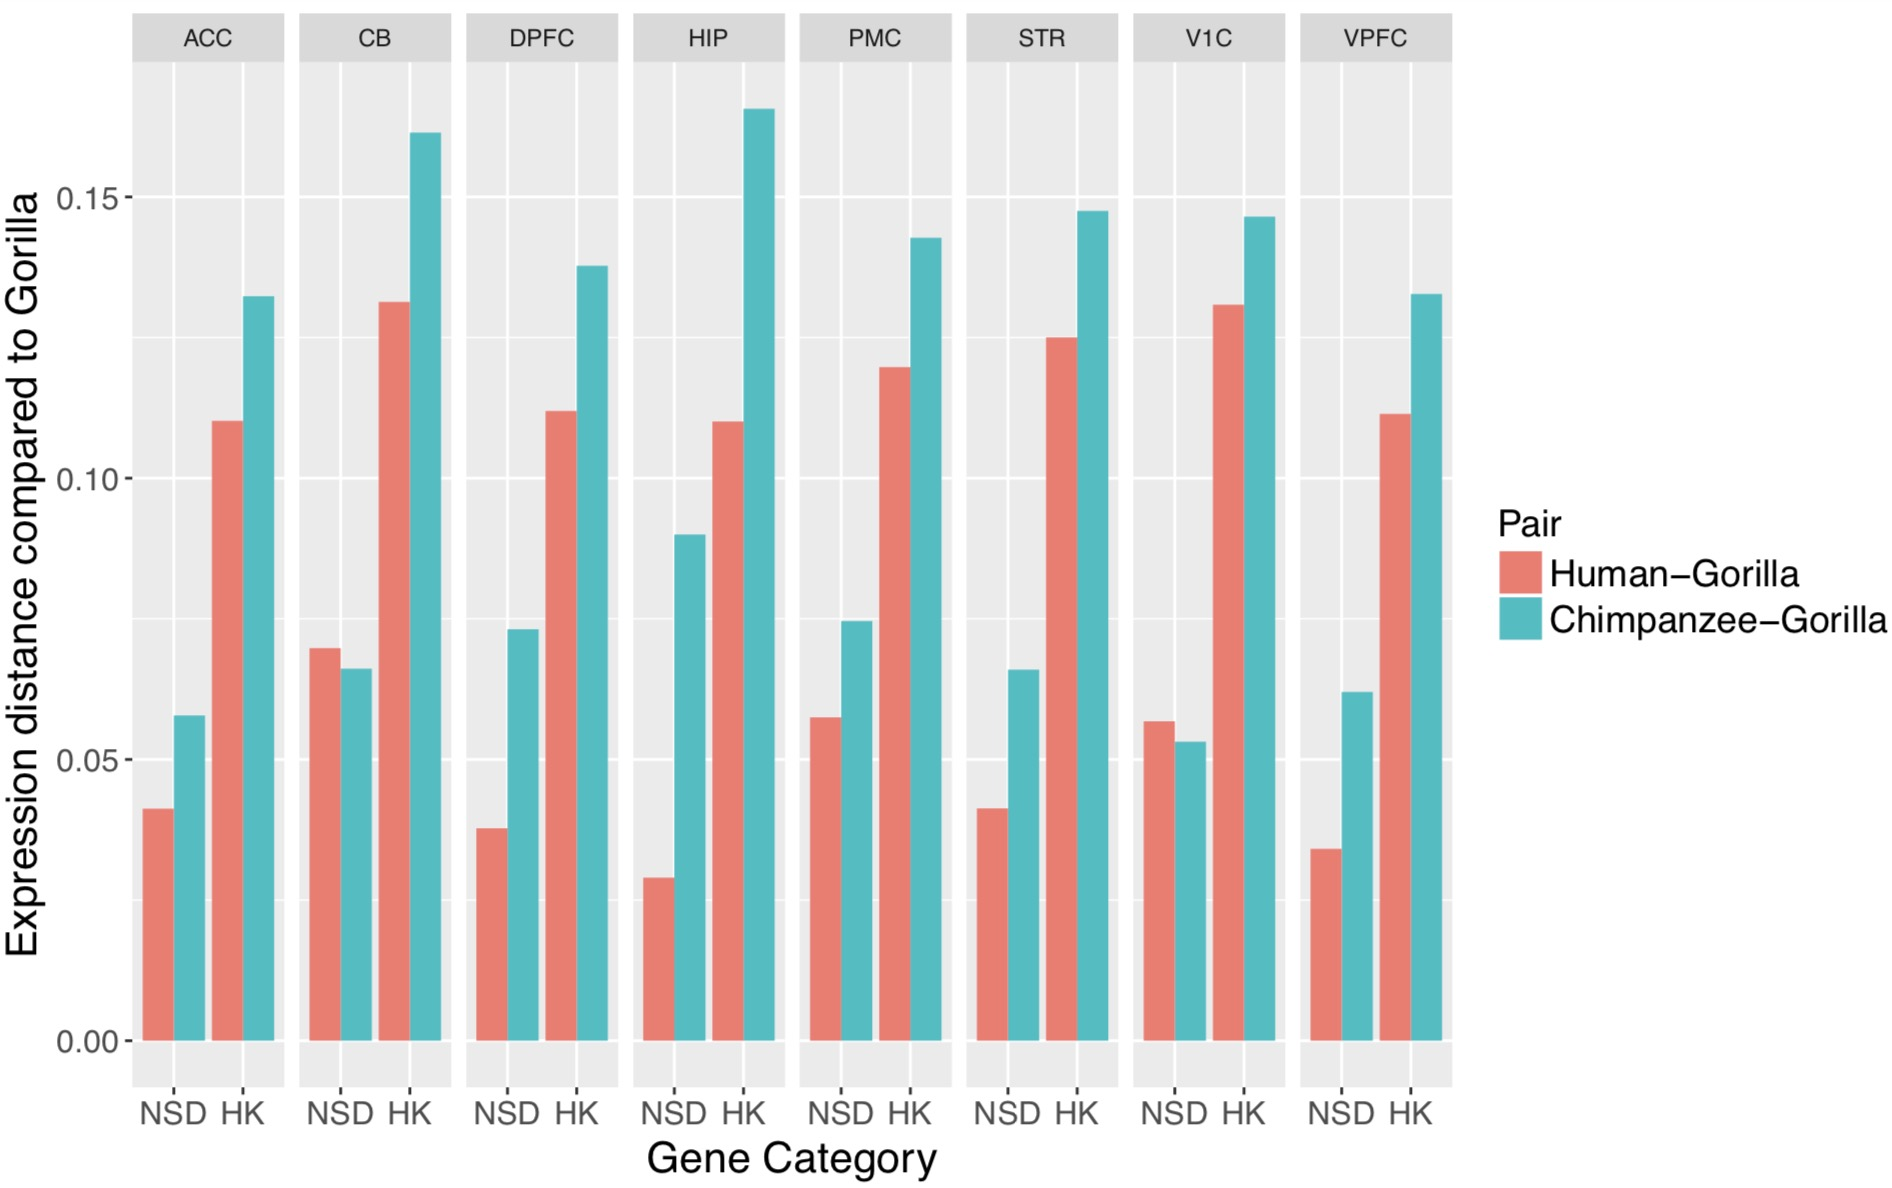
\includegraphics[width=0.8\textwidth,height=0.8\textwidth]{/blog/2018-10-15-灵长动物8脑区转录组进化分析_files/NSD-HK-Gorilla.jpg}
\caption{图七 human, chimpanzee相对gorilla在8个脑区中的表达进化距离}
\end{figure}

\end{document}
